\documentclass{article}
\usepackage{amsmath}
\usepackage{amssymb}
\usepackage{graphicx}
\usepackage[margin=1in]{geometry}
\usepackage{hyperref}
\usepackage{caption}
\usepackage{float}
\graphicspath{{images/}}
\hypersetup{
    colorlinks=true,
    urlcolor=blue,
}
\begin{document}

\title{The Plastic Field}
\author{Aresh Pourkavoos}
\maketitle

The plastic ratio $\rho$ is the real solution to $\rho^3 = \rho+1$,
with an approximate value of $1.3247$.
Its definition puts it into the set of numbers
that gives the golden ratio many of its interesting
(and, to some, mystical) properties: the algebraic integers.
A few quick facts:
\begin{itemize}
  \item
    Contrary to first impressions,
    the word ``plastic'' in this constant's name
    refers not to the material but to the idea of plasticity, or flexibility.
  \item
    It is the smallest of the PV numbers,
    which are the reals greater than 1
    whose powers approach integers.
    The powers of $\rho$ approach a sequence known as the Perrin numbers.
    (The golden ratio is also a PV number,
    and its powers approach the Lucas numbers,
    which are closely related to the Fibonacci numbers.)
  \item
    
\end{itemize}

My most recent encounter with this number
came from the uniform polyhedron known as
the snub icosidodecadodecahedron, or ``sided'' for short.

\begin{center}
  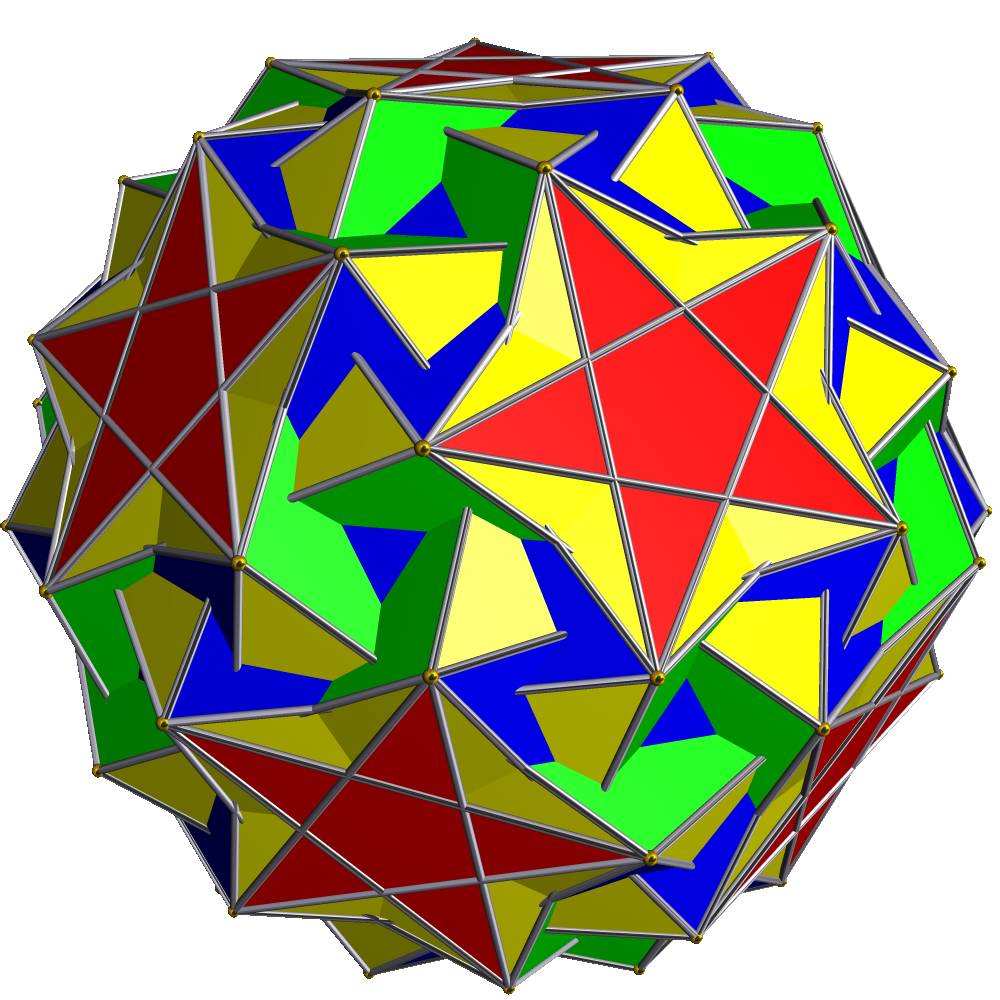
\includegraphics[width=0.25\linewidth]{sided.png} \\
  Created using \href{http://www.software3d.com/Stella.php}{Stella}
\end{center}

Like many polyhedra related to the icosahedron,
the coordinates of its vertices involve the golden ratio.
What surprised to me, however,
was the inclusion of the plastic ratio as well,
which does not appear in any other uniform polyhedra.
At a certain scale, its vertices may be written as follows,
where $\varphi$ is the golden ratio:

\begin{align*}
  & (2\alpha, 2\beta, 2\gamma), \\
  & (\alpha+\beta/\varphi+\gamma\varphi,
  -\alpha\varphi+\beta+\gamma/\varphi,
  \alpha/\varphi+\beta\varphi-\gamma), \\
  & (-\alpha/\varphi+\beta\varphi+\gamma,
  -\alpha+\beta/\varphi-\gamma\varphi,
  \alpha\varphi+\beta-\gamma/\varphi), \\
  & (-\alpha/\varphi+\beta\varphi-\gamma,
  \alpha-\beta/\varphi-\gamma\varphi,
  \alpha\varphi+\beta+\gamma/\varphi), \\
  & (\alpha+\beta/\varphi-\gamma\varphi,
  \alpha\varphi-\beta+\gamma/\varphi,
  \alpha/\varphi+\beta\varphi+\gamma),
\end{align*}
where
\begin{align*}
  \alpha &= \rho+1, \\
  \beta &= \varphi^2(\rho^2+\rho)+\varphi, \\
  \gamma &= \rho(\varphi+\rho).
\end{align*}

These 5 sets of coordinates form a single pentagrammic face of sided.
The 3 coordinates of each vertex are rotated to create 10 new triplets,
e.g. $(2\alpha, 2\beta, 2\gamma)$ yields
$(2\beta, 2\gamma, 2\alpha)$ and $(2\gamma, 2\alpha, 2\beta)$.
This represents a 120-degree rotation about the axis $x=y=z$,
and the image above is almost looking down on such a threefold symmetry axis,
running through the center of 3 pentagrams.
Next, even sign changes are applied,
meaning that that the 4 possible ways of negating none or two of the coordinates
represent vertices of sided,
bringing the total from 15 to 60, the actual number of vertices.
The even sign changes represent 180-degree rotations,
and the twofold symmetry axes around which these rotations are performed
may also be seen above, running between adjacent pentagrams.

\begin{align*}
  a+b\rho+c\rho^2 &\cong
  \begin{bmatrix}
    a & c & b \\
    b & a+c & b+c \\
    c & b & a+c
  \end{bmatrix} = M \\
  M^{-1} &= \frac{\mathrm{adj}(M)}{\lvert M \rvert} \\
  \mathrm{adj(M)} &=
  \begin{bmatrix}
    d & \\
    e & \hdots \\
    f &
  \end{bmatrix}
  \cong d+e\rho+f\rho^2 \\
  d &=
  \begin{vmatrix}
    a+c & b+c \\
    b & a+c
  \end{vmatrix}
  = (a+c)^2-b(b+c) \\
  e &=
  \begin{vmatrix}
    b+c & b \\
    a+c & c
  \end{vmatrix}
  = c^2-ab \\
  f &=
  \begin{vmatrix}
    b & a+c \\
    c & b
  \end{vmatrix}
  = b^2-(a+c)c \\
  \lvert M \rvert &= ad+ce+bf \\
  \frac{1}{a+b\rho+c\rho^2} &=
  \frac{d+e\rho+f\rho^2}{\lvert M \rvert} \\
\end{align*}

\end{document}
